\documentclass{book}
\usepackage{listings}
\usepackage{hyperref}
\usepackage{verbatim}
\usepackage{amsmath}
\usepackage[backend=bibtex, sorting=none, style=numeric-comp, defernumbers]{biblatex}
\usepackage{graphicx}

\addbibresource{\jobname.bib}

\title{Chapter 4 - Unsupervised Learning}
\author{Joydeep Bhattacharjee}

\begin{document}
\maketitle

In the previous chapters we took a look at the regression and classification algorithms which fall under the category of Supervised algorithms\cite{UL:1} . In this chapter we will be taking a look at Unsupervised algorithms. In unsupervised algorithms the labels or the target classes are not given. So the goal of unsupervised learning is to attempt to find natural partitions of patterns. 

The best time for unsupervised learning is when the data on desired outcomes is not known, such as creating a new class of products that the business has never sold before.

Some applications of unsupervised learning are listed below:

\begin{itemize}
	\item \textbf{Clustering} allows automatic splitting of the data set into groups according to a notion of similarity. Often, however, cluster analysis overestimates the similarity between groups and doesn't treat data points as individuals. For this reason, cluster analysis is a port choice for applications like customer segmentation and targeting.
	\item \textbf{Anomaly Detection} can automatically discover unusual data points in your dataset. This is useful in problems such as fraudulent transactions, discovering faulty pieces of hardware, or discovering an outlier in various processes.
	\item \textbf{Association Mining} identifies sets of items that frequently occur together in the data set. Retailers often use it for basket analysis, because it allows analysts to discover goods often purchased at the same time and develop more effective market strategies.
	\item \textbf{Latent Variable models} are commonly used in data preprocessing, such as reducing the number of features in a data set, otherwise known as dimensionality reduction, or decomposing the dataset into multiple components.
\end{itemize}
This chapter will focus on different unsupervised learning algorithms and how we can implement them using Rust. The code that we will look at can be found in the package \lstinline{rusty_machine_unsupervised} in the folder \lstinline{chapter2}. We will be using the same iris data set and the data preparation steps would be the same that we had seen in the regression chapter (Chapter 2). Finally we should have two rusty machine dense matrices \lstinline{flower_x_train} and \lstinline{flower_x_test}.

\section{KMeans clustering}%
K-means is one of the simplest unsupervised learning algorithms that solve the clustering problem. The idea is to classify a data set through a certain number of clusters fixed apriori. If the number of clusters are k then the objective is to define k centers, one for each cluster. There are different methods of choosing where the k centers should be. Take each point and associate it with the nearest cluster center. Once all the points are done then we update the cluster center to the center of the cluster of points that it has been associated with resulting in new $k$ cluster centers. The previous step is repeated for the new cluster centers and again each cluster center gets associated with a new subset of points. The centers are again updated based on the new sets. This back and forth updation of cluster centers and cluster sets are repeated till the stopping criteria is met. The stopping criteria can either be a fixed number of iterations or if the change in the cluster centers fall below a threshold. This algorithm aims at minimizing an objective function

\begin{equation}
	J(V) = \sum_{i=1}^{C}\sum_{j=1}^{C_i}(||x_i - \nu_j||)^2
\end{equation}

where, $||x_i - v_j||$ is the Euclidean distance between $x_i$ and $v_j$, $c_i$ is the number of data points in the $i^{th}$ cluster and $c$ is the number of cluster centers.

Commonly used initialization patterns are Forgy, Random partition and KMeans++. The Forgy method randomly chooses k observations from the data set and uses them as the initial means. The random partition method first randomly assigns a cluster to each observation and then proceeds to the update step, thus computing the initial mean to be the centroid of the cluster's randomly assigned points. The Forgy method tends to spread the initial means out, while Random partition places all of them close to the center of the data set.

KMeans++ is almost the same as vanilla KMeans just that Kmeans++ starts with allocating one cluster center randomly and then searches for other centers given the first one. To show how this works let D(x) denotes the shortest distance from a data point to the closest center we have already chosen\cite{UL:10}.

\begin{enumerate}
	\item Take one center $c_1$, chosen uniformly at random from $\chi$.
	\item Take a new center $c_i$, choosing $x \in \chi$ with probability $\frac{D(x)^2}{\sum_{x \in \chi}^{D(x)^2}}$
	\item Repeat the previous step until we have $k$ centers altogether.
	\item Proceed with the standard k-means algorithm.
\end{enumerate}

Using \lstinline{rusty-machine} we can use the \lstinline{KMeansClassifier} struct to implement apply KMeans on the data using the \lstinline{train} method. We can then either see the model centroids or run the predict method on the unseen data.

\begin{lstlisting}[caption={rusty\_machine\_unsupervised}]
use rusty_machine as rm;
use rm::learning::k_means::KMeansClassifier;

let mut model = KMeansClassifier::new(clusters);
model.train(&flower_x_train)?;
let centroids = model.centroids().as_ref().unwrap();
println!("Model Centroids:\n{:.3}", centroids);

println!("Predicting the samples...");
let classes = model.predict(&flower_x_test).unwrap();
println!("number of classes from kmeans: {:?}",
  classes.data().len());
\end{lstlisting}

Creating the above model initialises the k-means using kmeans$++$. Apart from this we can also use the Forgy or RandomPartition method.

\begin{lstlisting}[caption={rusty\_machine\_unsupervised}]
use rm::learning::k_means::{KMeansClassifier, Forgy,
                            RandomPartition, KPlusPlus};
// can use either Forgy or RandomPartition
let mut model = KMeansClassifier::new_specified(3, 100, Forgy);
\end{lstlisting}

where $3$ is the number of partitions and the number of epochs is kept at $100$.

\label{sec:kmeans_clustering}
\section{Gaussian Mixture Model}%
K-means and the associated expectation-maximization algorithm, is a special case of the Gaussian mixture model. The k-means clustering explored in the previous section is simple and relatively easy to understand, but its simplicity leads to practical challenges in its application. In particular, the non probabilistic nature of k-means and its use of simple distance-from-cluster-center to assign cluster membership leads to poor performance for many real world situations. In this section we will take a look at Gaussian Mixture Models (GMMs), which can be viewed as an extension of the ideas behind k-means, but can also be a powerful tool for estimation behind simple clustering \cite{UL:7} 

One way to think about the k-means model is that it places a circle sphere of influence (or a circle for the simplest case) at the center of each cluster, with a radius defined by the most distant points in the cluster. This radius acts as the hard cutoff for the cluster assignment within the training set: any point outside the circle is not considered a member of the cluster.

Note an important point. Because the k-means considers the points belonging to a cluster on the basis of a definition of nearness, these "spheres of influence" must be circular. A better model might be accounting for distributions where the distribution might be of a different shape. In GMMs the k-means is generalized to a probabilistic model where we assume that all the data points are generated from a mixture of a finite number of Gaussian distributions with unknown parameters.

The multivariate Gaussian distribution of an n-dimensional vector $x = (x_1, x_2, ..., x_n)$ may be written as

\begin{equation}
	p(x; \mu, \Sigma) = \frac{1}{\sqrt{(2\pi)^n |\Sigma|}} \text{exp}(- \frac{1}{2}(x - \mu)^T\Sigma^{-1}(x - \mu))
\end{equation}

where $\mu$ is the n-dimensional mean vector and $\Sigma$ is the $n x n$ covariance matrix. Below is a figure to simulate the possible Gaussian distribution for a distribution.

\begin{figure}[htpb]
	\centering
	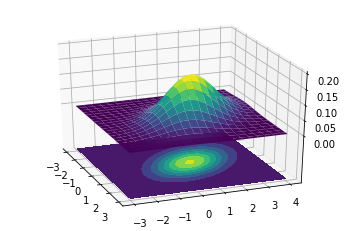
\includegraphics[width=0.8\linewidth]{gaussian_dist.png}
	\caption{Gaussian}
	\label{fig:gaussian}
\end{figure}

In the below picture we are using the iris dataset to map distribution between two variables \lstinline{sepal_length} and \lstinline{sepal_width}.

\begin{figure}[htpb]
	\centering
	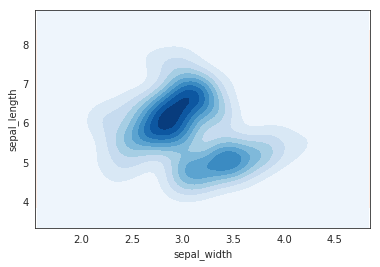
\includegraphics[width=0.8\linewidth]{multiple_contours.png}
	\caption{multiple distributions}
	\label{fig:multiple_distributions}
\end{figure}

A Gaussian distribution is completely determined by its covariance matrix and its mean. The covariance matrix of a Gaussian distribution determines the directions and lengths of the aces of its density contours, all of which are ellipsoids. The different type of covariance matrices are

\begin{itemize}
	\item \textbf{Full} means that the components may independently adopt any position and shape.
	\item \textbf{Tied} means they have the same shape but the shape may be anything.
	\item \textbf{Diagonal} means that the contour axes are oriented along the coordinate axes, but otherwise the eccentricities may vary between components.
	\item \textbf{Spherical} means that the contour is a sphere.
	\item \textbf{Toeplitz} means that the diagonals of the contour has elements that share the same paramters. It has an additional complexity parameter that selects the number of active off-diagonals and their constants.
	\item \textbf{Shrinked} means that the contour shape is determined by the complex combination of a diagonal and any covariance. No immediate obvious tying, but ties all eigenvalues so that they grow and shrink depending on the same parameter.
	\item \textbf{Kernel covariance}, in this case the covariance is defined by a positive definite function. We are in this case able to get a mixture model of functions (the greatest amount of generalisation mathematically speaking).
\end{itemize}

Apart from the above, constraints can be put on the Gaussian mixture composition, which increases generalisation of the model\cite{UL:8}.

\paragraph{EM algorthm}%
Finding the Gaussian Mixtures is computationally expensive and hence we resort to the Expectation Maximisation algorithm. Expectation Maximisation is an iterative method to find maximum likelihood estimates of parameters in statistical models, where the model depends on unobserved latent variables. In this case we can think of the mixing probabilities of the Gaussian functions as the prior probabilities for the components. For given input values of the individual components, we can evaluate the corresponding posterior probabilities, called responsibilities. These responsibilities are essentially the latent variables\cite{UL:3} .

So we resort to the EM algorithm. We define the EM-algorithm for Gaussian Mixture as an iterative algorithm that starts from some initial estimate of the parameters ${\mu, \Sigma}$ (e.g random), and then proceeds to iteratively update the parameters until convergence is achieved. Each iteration consists of an E-step and an M-step.

\textbf{E-Step}: For the given parameter values we can compute the expected values of the latent variables, in this case the responsibilities.

\begin{equation}
	\hat{\gamma_i} = \frac{\hat{\pi}\phi_{\hat{\theta_2}}(y_i)}{(1 - \hat{\pi})\phi_{\hat{\theta_1}}(y_i) + \hat{\pi}\phi_{\hat{\theta_2}} \cdot (y_i)}, i = 1, 2, ..., N
\end{equation}

\textbf{Maximisation step}: In this case we update the parameters of the model based on the latent variable calculated using the ML method.

\begin{equation}
	\hat{\mu_1} = \frac{\Sigma_{i=1}^{N}(1 - \hat{\gamma_i}) y_i}{\Sigma_{i=1}^{N}(1 - \hat{\gamma_i})}, \\
	\hat{\sigma_1} = \frac{\Sigma_{i=1}^{N}(1 - \hat{\gamma_i}) (y_i - \hat{\mu_i})^2}{\Sigma_{i=1}^{N}(1 - \hat{\gamma_i})}, \\
	\hat{\mu_2} = \frac{\Sigma_{i=1}^{N}\hat{\gamma_i} y_i}{\Sigma_{i=1}^{N}\hat{\gamma_i}}, \\
	\hat{\sigma_2} = \frac{\Sigma_{i=1}^{N}\hat{\gamma_i} (y_i - \hat{\mu_i})^2}{\Sigma_{i=1}^{N}\hat{\gamma_i}}, \\
\end{equation}
and the mixing probability $\hat{\pi} = \Sigma_{i=1}^{N}\frac{\hat{\gamma_i}}{N}$.
\label{par:em_algorthm}


The above steps will be iterated till stopping criteria or convergence.

\paragraph{Rust}%
Using \lstinline{rusty-machine}, we can create a mixture model. Then we set the maximum number of iterations and the covariance types. We can then train this model using the \lstinline{train} method. Once training is done apart from the \lstinline{predict} method we will also be able to get the means and the covariances of the trained model and run the predict method.

\begin{lstlisting}[caption={rusty\_machine\_unsupervised}]
let mut model = GaussianMixtureModel::new(2);
model.set_max_iters(1000);
model.cov_option = CovOption::Diagonal;

println!("Training the model");
model.train(&flower_x_train)?;

// Print the means and covariances of the GMM
println!("{:?}", model.means());
println!("{:?}", model.covariances());

// Predict the classes and partition into
println!("Predicting the samples...");
let classes = model.predict(&flower_x_test).unwrap();
println!("number of classes from GMM: {:?}", classes.data().len());
\end{lstlisting}

In place of \lstinline{Diagonal}, we can also use the \lstinline{Full} and \lstinline{Regularized} options.`
\label{par:rust}





% http://ethen8181.github.io/machine-learning/clustering/GMM/GMM.html
% https://www.quora.com/When-learning-the-covariance-matrices-of-a-Gaussian-mixture-model-what-are-different-types-of-parameter-tying
% https://athemathmo.github.io/rusty-machine/doc/rusty_machine/learning/gmm/index.html
% http://www.cse.iitm.ac.in/~vplab/courses/DVP/PDF/gmm.pdf
% https://www.youtube.com/watch?v=JNlEIEwe-Cg
% http://statweb.stanford.edu/~tibs/stat315a/LECTURES/em.pdf

\label{sec:gaussian_mixture_model}

\section{Density Based Spatial Clustering of Applications with Noise}%
The DBSCAN algorithm views clusters as areas of high density separated by areas of low density. Due to this generic view, clusters found by DBSCAN can have any shape, as opposed to k-means which assumes that clusters are convex shape. Clusters are identified by looking at the density of points. Regions with a high density of points depict the existence of clusters whereas regions with a low density of points indicate clusters of noise or clusters of outliers. This algorithm is particularly suited to large data sets, with noise, and is able to identify clusters with different sizes and shapes.

The main concept of DBSCAN is that of core-samples, meaning that for each point of a cluster, the neighbourhood of a given radius has to contain atleast a minimum number of points, or in other words, the "density" in the neighbourhood has to exceed some predefined threshold. This algorithm needs three input parameters\cite{UL:9}.

\begin{itemize}
	\item k, the nearest neighbour list size.
	\item eps, the radius that delimit the neighbourhood area of a point.
	\item min points, the minimum number of points that must exist in the eps-neighbourhood.
\end{itemize}

To below are the steps that the DBSCAN algorithm uses.

\begin{enumerate}
	\item To cluster a data set, our DBSCAN implementation starts by identifying the k nearest neighbours of each point and identifying the k nearest neighbours of each point and identify the farthest k nearest neighbour. The average of all this distance is then calculated.
	\item For each point of the data set the algorithm identifies the directly density-reachable points using the eps threshold provided by the user and classifies the points into core or border points.
	\item It then loops through all the points of the data set and for the core points it starts to construct a new cluster by following the definition of density reachable points.
\end{enumerate}

At the end the composition of the clusters is verified to check if there exists clusters that can be merged together. This is done when two clusters are at a distance less than eps.

The issues with DBSCAN is that it cannot handle varying densities. Also this algorithm is quite sensitive to parameters set.

DBSCAN models can be created using rusty-machine. In the below code we create a DBSCAN model with eps as $3$ and minimum samples as $10$. We then pass \lstinline{true} to \lstinline{set_predict} method of the model. This allows us to use the \lstinline{predict} on new unseen data. Similar to previous models we can train and predict on the data set. Apart from these we can also check the clusters which the model has learned.

\begin{lstlisting}[caption={rusty\_machine\_unsupervised}]
use rm::learning::dbscan::DBSCAN;
use rm::learning::UnSupModel;
let mut model = DBSCAN::new(0.3, 10);
model.set_predictive(true);

model.train(&flower_x_train)?;

let clustering = model.clusters().unwrap();

let classes = model.predict(&flower_x_test).unwrap();
\end{lstlisting}

Apart from \lstinline{DBSCAN::new} we can use \lstinline{DBSCAN::default}. The default values that are initialized are $0.5$ for eps, $5$ for minimum points.

\label{sec:dbscan}

\section{Principal Component Analysis}%
One of the main components of machine learning is matrix multiplication. Matrix multiplications are generally computationally expensive\cite{UL:4}. Also the number of dimensions that we are dealing with needs to be taken into account and we should not add too many dimensions unnecessarily. We are shown by the Hughes phenomenon that as the number of features increases, a classifiers performance increases as well until we reach the optimal number of features. Adding more features for the same size as the training set will degrade the features. This is called the curse of dimensionality\cite{UL:5}.

\begin{figure}[htpb]
	\centering
	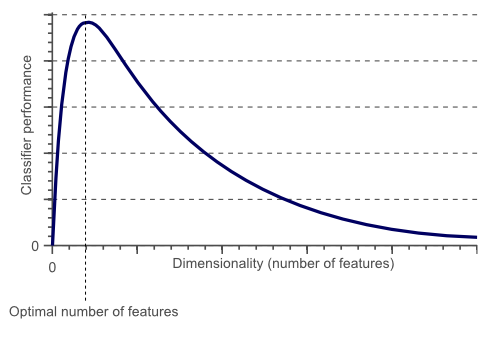
\includegraphics[width=0.8\linewidth]{HughesPhenomenon.png}
	\caption{Hughes Phenomenon}
	\label{fig:Hughes_Phenomenon}
\end{figure}

Many algorithms such as KNN are particularly susceptible to this curse of dimensionality. A way to escape this curse is by dimensionality reduction. In dimensionality reduction we generally choose a mathematical representation within which most of the variance in the original data, if not all, can be explained. The effect is that we are able to remove a significant number of features while retaining a lot of the information.

Principal Component Analysis is a method of dimensionality reduction. Its essentially a transformation where our original variables will get converted to a new set of variables, which are linear combinations of the original set of variables. In other words

\begin{equation}
	PX = Y
\end{equation}

where X is the original recorded data set, Y is the representation of the data set and P is the linear transformation matrix. Geometrically we can see that P is a rotation and stretch from $X$ to $Y$.

To understand PCA we will need to look into the concept of covariance. The covariance measures the degree of the linear relationship between two variables and is given by

\begin{equation}
	\text{covariance of two variables A and B} \equiv \sigma_{AB}^2 = \frac{1}{n - 1}AB^T
\end{equation}

where division by $n - 1$ is for normalization. We can now generalize from A and B to an arbitrary matrix X and define the covariance matrix C as.

\begin{equation}
	C_X = \frac{1}{n - 1}XX^T
\end{equation}

Important properties of $C_X$ are:

\begin{itemize}
	\item $C_X$ is a square symmetric $m \times m $ matrix.
	\item The diagonal terms of $C_X$ are the variance of particular measurement types.
	\item The off-diagonal terms of $C_X$ are the covariance between measurement types.
\end{itemize}

High diagonal values means that the different measurements are highly correlated and we don't need to take so many different measurements of a single event. A way to write this is for some orthonormal matrix $P$ where $Y = PX$ such that $C_Y = \frac{1}{n - 1}YY^T$ is diagonalized. The rows of P are the principal components.

In practice computing PCA of a data set X entails substracting off the mean of each measurement type and computing the eigenvectors of $XX^T$.

Now given a set of measurements PCA works by the following logic. It assumes that all basis vectors ${p_1, p_2, \ldots, p_m}$ are orthonormal. In multiple dimensions the PCA can be given by the below algorithm

 \begin{enumerate}
 	\item We select a normalized direction in m-dimensional space along which the variance in X is maximized. Save this vector as $p_1$
 	\item We select another direction along which variance is maximized, however, because of the orthonormality condition, restrict the search to all directions perpendicular to all previous directions. 
 	\item Repeat this procedure till m vectors are selected.
 \end{enumerate}

The resultant ordered sets of p's are the principal components.

\paragraph{Singular Value Decomposition}%
Most software packages implement PCA using Singular Value Decomposition (or SVD). SVD is a general way to understand a matrix in terms of its column space and row-space. In this we decompose a matrix into three other matrices

\begin{equation}
	A = USV^T
\end{equation}

On similar lines we can decompose the previous X matrix using SVD,

\begin{equation}
	X = U \Gamma V^T
\end{equation}

and then write the covariance matrix as

\begin{equation}
	C = \frac{1}{n}XX^T = \frac{1}{n}U\Gamma^2U^T
\end{equation}

In this case U is an $n \times m$ matrix. Following the fact that SVD routine order the singular values in descending order we know that, if n < m, the first n columns in U corresponds to the sorted eigenvalues of C and if $m \geq n$, the first m corresponds to the sorted non-zero eigenvalues of C. The transformed data can thus be written as
\begin{equation}
	Y = \hat{U^T}X = \hat{U^T}U \Gamma V^T
\end{equation}

where $\hat{U^T}U$ is a simple $n \times m$ matrix which is one on the diagonal and zero everywhere else. To conclude, we can write the transformed data in terms of the SVD decomposition of X\cite{UL:6}.

\label{par:singular_value_decomposition}

\paragraph{PCA and Rust}%
Although PCA has been implemented in \lstinline{rusty-machine}, it has not been published in the crate as of the writing of this book. Hence we will need to update the dependencies in Cargo.toml file to pull in the latest code from the master

\begin{lstlisting}[caption={Cargo.toml}]
[dependencies]
rusty-machine = { git = "https://github.com/AtheMathmo/rusty-machine.git", rev = "f43da8d" }
\end{lstlisting}

Now we should be able to create a PCA model and train on the data. In this case we are reducing the dimensions to 2 and ask the model to center the clusters.

\begin{lstlisting}[caption={rusty\_machine\_unsupervised}]
use rm::learning::pca::PCA;
use rm::learning::UnSupModel;
let mut model = PCA::new(2, true);
model.train(&flower_x_train)?;

println!("{:?}", model.predict(&flower_x_test)?);
println!("{:?}", model.components());
\end{lstlisting}

We can also use the \lstinline{PCA::default} method to create a default model, but the default model has all the components. So we will not be having reduction in the dimensions then.

\label{par:pca_and_rust}



% https://www.cs.cmu.edu/~elaw/papers/pca.pdf

\label{sec:principal_component_analysis}

\section{Testing an Unsupervised model}%
Evaluating the performance of an unsupervised model is difficult as there are no labels to compare the final score with. One way is through internal metrics such as the silhouette score, which aims at formalizing the attainment of high intra-cluster similarity, or points within a cluster should be close to each other and low inter-cluster similarity which means similarity between points in two clusters should be low. But good scores on an internal criterion may not necessarily translate into good effectiveness in application. The other approach is through direct evaluation in the application of interest. For example a website implementing search may measure the time taken by the users to find an answer with different clustering algorithms and the two algorithms can be compared with beta testing. This is the most direct evaluation, but it is expensive, especially if large user studies are necessary.

A third approach by using a surrogate of user judgements, in which case we use a set of classes and create a gold standard ourselves. The gold standard is ideally produced by human judges with good level of inter-judge agreement. We can then compute an external criterion that evaluates how well the cluster matches the gold standard classes. In this section two measures of external criteria are described with code accompanying them.

\paragraph{Rand Index}%
The Rand Index computes a similarity measure between two clusterings by considering all pairs of samples and counting pairs that are assigned in the same or different clusters in the predicted and true clusterings. The most common formulation of he Rand index focuses on the following four sets of the $\binom nk$ element pairs:: $N_{11}$ is the number of element pairs that are grouped in the same cluster in both clusterings, $N_{10}$ is the number of element pairs which are grouped in the same cluster by $A$ but in different clusters by $B$, $N_{01}$ the number of element pairs which are grouped in the same cluster by $B$ but in different clusters by $A$, and $N_{00}$ the number of elements pairs which are grouped in different clusters by both $A$ and $B$. Notice that $N_{11}$ and $N_{00}$ are the indicator of agreements between clusters $A$ and $B$ while $N_{10}$ and $N_{01}$ are the disagreements.

\begin{table}[htpb]
	\centering
	\caption{contingency table}
	\label{tab:label}
	\begin{tabular}{|l|l|l|l|l|l|}
            $A$/$B$ & $B_1$    & $B_2$    & \dots  & $B_n$    & Sums  \\ \hline
            $A_1$   & $n_{11}$ & $n_{12}$ & \dots  & $n_{1n}$ & $a_1$ \\
            $A_2$   & $n_{21}$ & $n_{22}$ & \dots  & $n_{2n}$ & $a_2$ \\
            $\vdots$  & $\vdots$   & $\vdots$   & $\vdots$ & $\vdots$   & $\vdots$ \\
            $A_n$   & $n_{n1}$ & $n_{n2}$ & $\ddots$ & $n_{nn}$ & $a_n$ \\ \hline
            Sums    & $b_1$    & $b_2$    & $\dots$  & $b_n$    & $N$
	\end{tabular}
\end{table}

The contingency is shown in table 1. Therefore the rand index would be given by the below function

\begin{equation}
	RI(A, B) = \frac{N_{11} + N_{00}}{\binom nk}
\end{equation}

The value of the above index would lie between 0 and 1, where 1 indicates that the clusterings are identical and 0 means that the clusters do not share a single pair of elements.

Rand index is implemented in \lstinline{ml-utils}.

\begin{lstlisting}[caption={ml\\-utils\\/src\\/unsup\_metrics\\.rs}]
pub fn rand_index(clusters1: &[HashSet<u64>],
    clusters2: &[HashSet<u64>]) -> f64 {
  let (n11, n10, n01, n00) = count_pairwise_cooccurence(
    clusters1, clusters2);
  (n11 + n00) / (n11 + n10 + n01 + n00)
}
\end{lstlisting}

The implementation of \lstinline{count_pairwise_cooccurence} function can be found on the same module and has been skipped for brevity.

We should now be able to run this function and get the index.

\begin{lstlisting}[caption={ml\\-utils\\/src\\/unsup\_metrics\\.rs}]
use ml_utils::unsup_metrics::rand_index;

println!("rand index: {:?}",
  rand_index(&predicted_clusters, &flower_y_test_clus));
\end{lstlisting}

\label{par:rand_index}

\paragraph{Jaccard Index}%
Similar to the rand index we have the jaccard index. It is defined by the size of the intersection divided by the size of the union.

\begin{equation}
	J(A, B) = \frac{|A \cap B|}{|A \cup B|}
\end{equation}

This can be easily understood by the figure: 4. The intersection should approach the union as the clusters are similar to each other.

\begin{figure}[]
	\centering
	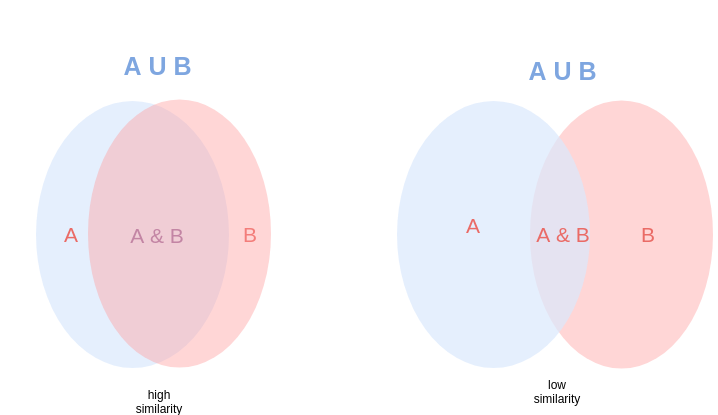
\includegraphics[width=0.8\linewidth]{jaccard.png}
	\caption{Jaccard}
	\label{fig:jaccard}
\end{figure}

Take a look at the implementation of jaccard index in \lstinline{ml-utils}.

\begin{lstlisting}[caption={ml\\-utils\\/src\\/unsup\_metrics\\.rs}]
pub fn jaccard_index(clusters1: &[HashSet<u64>],
    clusters2: &[HashSet<u64>]) -> f64 {
  let (n11, n10, n01, n00) = count_pairwise_cooccurence(clusters1, clusters2);
  let denominator = n11 + n10 + n01;
  if denominator > 0.0 {
    return n11 / denominator;
  } else {
    0.0
  }
}
\end{lstlisting}

We should now be able to run this function and get the index.

\begin{lstlisting}[caption={ml\\-utils\\/src\\/unsup\_metrics\\.rs}]
use ml_utils::unsup_metrics::jaccard_index;

println!("jaccard index: {:?}",
  jaccard_index(&predicted_clusters, &flower_y_test_clus));
\end{lstlisting}

\label{par:jaccard_index}

% https://medium.com/hockey-stick/tl-dr-bayesian-a-b-testing-with-python-c495d375db4d
% https://towardsdatascience.com/the-math-behind-a-b-testing-with-example-code-part-1-of-2-7be752e1d06f
% https://nlp.stanford.edu/IR-book/html/htmledition/evaluation-of-clustering-1.html
% find ways to give similarity scores https://github.com/Hoosier-Clusters/clusim/tree/master/clusim

\label{sec:testing_an_unsupervised_model}

\section{Conclusion}%
This chapter introduced you to different algorithms for unsupervised learning such as Kmeans clustering, Gaussian Mixture models, DBSCAN models and Principal Component Analysis. We also took a look at how to create these models using \lstinline{rusty_machine} library. Finally you got to know about evaluating unsupervised models using rand index and jaccard index.

In the next chapter you will learn about working with data and how to create effective data pipelines in Rust.
\label{sec:conclusion}



\printbibliography
\nocite{*}
\end{document}
